\documentclass[aspectratio=169]{beamer}

% Shared Beamer settings for Applied Machine Learning lectures (UPES).
% Keep this file free of \documentclass to allow reuse via \input.

% Allow lecture sources to use shared theme/assets without copying them into each lecture folder.
% NOTE: These paths are relative to `Unit-xx/Lecture-yy/latex/` (and `Lab/Experiment-xx/latex/`).
\makeatletter
\def\input@path{{../../../_shared/}{../../../_shared/UPES-Beamer-Theme/}}
\makeatother

\usetheme{UPES}
\setbeamertemplate{navigation symbols}{}

\usepackage{amsmath}
\usepackage{amssymb}
\usepackage{booktabs}
\usepackage{graphicx}
\usepackage{hyperref}
\usepackage{xcolor}
\usepackage{listings}

% Code listings (Python-oriented for this subject).
\lstset{
  language=Python,
  basicstyle=\ttfamily\small,
  keywordstyle=\color{blue},
  commentstyle=\color{gray},
  stringstyle=\color{teal},
  showstringspaces=false,
  columns=fullflexible,
  breaklines=true
}

\usepackage{tikz}
\usetikzlibrary{arrows.meta,positioning,shapes.geometric,calc,fit,backgrounds}

% Per-slide source line (references shown on the slide itself).
\newcommand{\slidesources}[1]{%
  \vfill
  {\tiny\color{gray}\raggedright\sloppy\parbox{\linewidth}{Sources: #1}\par}%
}

% Unit-wise source strings for this subject (used by slides/notes).
% Path is relative to the lecture `latex/` folder (the compilation CWD).
% Source strings for Applied Machine Learning (CSAI2017P) — used by slides + notes.
% Prescribed texts and reference books are taken from the course syllabus.
% Support texts are the author-hosted open-access editions:
%   statlearning.com            (ISL with Python)
%   probml.github.io/pml-book   (Murphy, Probabilistic Machine Learning)
%   d2l.ai                      (Dive into Deep Learning)
%   mml-book.github.io          (Mathematics for Machine Learning)

\newcommand{\AMLRepoURL}{https://github.com/tali7c/Applied-Machine-Learning}

% --- prescribed -------------------------------------------------------------
\newcommand{\AMLPrescribed}{%
M\"uller and Guido, \textit{Introduction to Machine Learning with Python}, O'Reilly, 2016.;%
Bishop, \textit{Pattern Recognition and Machine Learning}, Springer, 2006.;%
Murphy, \textit{Machine Learning: A Probabilistic Perspective}, MIT Press, 2012.;%
Han, Kamber and Pei, \textit{Data Mining: Concepts and Techniques} (3e), Morgan Kaufmann, 2012.%
}

% --- unit-wise ---------------------------------------------------------------
\newcommand{\AMLUnitISources}{%
M\"uller and Guido, \textit{Introduction to Machine Learning with Python}, Ch. 1.;%
Bishop, \textit{Pattern Recognition and Machine Learning}, Ch. 1.;%
Murphy, \textit{Probabilistic Machine Learning: An Introduction}, MIT Press, 2022, Ch. 1.;%
Mitchell, \textit{Machine Learning}, McGraw Hill, 1997, Ch. 1.;%
Scikit-learn documentation, accessed 2026-08-04.%
}

\newcommand{\AMLUnitIISources}{%
Bishop, \textit{Pattern Recognition and Machine Learning}, \S1.5, \S4.3, \S7.1.;%
Zhang, Lipton, Li and Smola, \textit{Dive into Deep Learning}, \S3.4.;%
Shalev-Shwartz and Ben-David, \textit{Understanding Machine Learning}, Ch. 15.;%
Murphy, \textit{Probabilistic Machine Learning: An Introduction}, Ch. 5.%
}

\newcommand{\AMLUnitIIISources}{%
Zhang, Lipton, Li and Smola, \textit{Dive into Deep Learning}, Ch. 12 (Optimization Algorithms).;%
Deisenroth, Faisal and Ong, \textit{Mathematics for Machine Learning}, Ch. 7.;%
Kingma and Ba, ``Adam: A Method for Stochastic Optimization,'' ICLR 2015.;%
Ruder, ``An overview of gradient descent optimization algorithms,'' arXiv:1609.04747, 2016.%
}

\newcommand{\AMLUnitIVSources}{%
Han, Kamber and Pei, \textit{Data Mining: Concepts and Techniques} (3e), Ch. 3.;%
M\"uller and Guido, \textit{Introduction to Machine Learning with Python}, Ch. 3--4.;%
James, Witten, Hastie, Tibshirani and Taylor, \textit{An Introduction to Statistical Learning with Python}, Ch. 5--6, 12.;%
Scikit-learn documentation (preprocessing, model selection), accessed 2026-08-04.%
}

\newcommand{\AMLUnitVSources}{%
James et al., \textit{An Introduction to Statistical Learning with Python}, Ch. 3--6.;%
Bishop, \textit{Pattern Recognition and Machine Learning}, Ch. 3.;%
Deisenroth, Faisal and Ong, \textit{Mathematics for Machine Learning}, Ch. 9.;%
M\"uller and Guido, \textit{Introduction to Machine Learning with Python}, \S2.3.%
}

\newcommand{\AMLUnitVISources}{%
Han, Kamber and Pei, \textit{Data Mining: Concepts and Techniques} (3e), Ch. 8--9.;%
James et al., \textit{An Introduction to Statistical Learning with Python}, Ch. 8--9.;%
Bishop, \textit{Pattern Recognition and Machine Learning}, Ch. 4--5, 7, 14.;%
Zhang et al., \textit{Dive into Deep Learning}, Ch. 5.%
}

\newcommand{\AMLUnitVIISources}{%
Han, Kamber and Pei, \textit{Data Mining: Concepts and Techniques} (3e), Ch. 10.;%
James et al., \textit{An Introduction to Statistical Learning with Python}, Ch. 12.;%
M\"uller and Guido, \textit{Introduction to Machine Learning with Python}, \S3.5.;%
Ester, Kriegel, Sander and Xu, ``A density-based algorithm for discovering clusters (DBSCAN),'' KDD 1996.%
}

\newcommand{\AMLLabSources}{%
M\"uller and Guido, \textit{Introduction to Machine Learning with Python}, companion notebooks.;%
McKinney, \textit{Python for Data Analysis} (3e), O'Reilly, 2022.;%
Scikit-learn user guide, accessed 2026-08-04.;%
Matplotlib and Seaborn documentation, accessed 2026-08-04.%
}



\graphicspath{{../figures/}{../images/}{../../../_shared/}{../../../_shared/UPES-Beamer-Theme/}}

\title[Applied Machine Learning]{Applied Machine Learning}
\subtitle{Unit 06 -- Lecture 19: Classification Model Evaluation:
          ROC and AUC}
\author{Tofik Ali}
\institute{School of Computer Science, UPES Dehradun}
\date{Autumn 2026}

% ---- a compact "output" block so code and its result sit together ----------
\lstdefinestyle{outblk}{
  basicstyle=\ttfamily\scriptsize\color{black!75},
  backgroundcolor=\color{black!5}, frame=leftline, framerule=2pt,
  rulecolor=\color{black!30}, breaklines=true, columns=fullflexible,
  keepspaces=true,   % several outputs below are aligned tables
  language={},       % printed output is not Python: do not syntax-highlight it
  xleftmargin=4pt, aboveskip=1pt, belowskip=1pt, literate={-}{{-}}1}
\lstnewenvironment{outblk}{\lstset{style=outblk}}{}

\newcommand{\TP}{\mathrm{TP}}
\newcommand{\FP}{\mathrm{FP}}
\newcommand{\TN}{\mathrm{TN}}
\newcommand{\FN}{\mathrm{FN}}
\newcommand{\TPR}{\mathrm{TPR}}
\newcommand{\FPR}{\mathrm{FPR}}

\begin{document}

\UPESCoverFrame
\setcounter{framenumber}{0}

\begin{frame}
  \titlepage
  \begin{center}
    \footnotesize The last lecture of the unit, and the one that decides which
    of the others you use\\[0.25em]
    \footnotesize Topic focus: \textbf{a classifier outputs a score, not a
    class}\\[0.25em]
    \footnotesize Repository: \texttt{\AMLRepoURL}
  \end{center}
  \slidesources{\AMLUnitVISources}
\end{frame}

\begin{frame}{Quick Links}
  \centering
  \hyperlink{sec:whynot}{\beamerbutton{Why not accuracy}}\hspace{0.4em}
  \hyperlink{sec:cm}{\beamerbutton{Confusion matrix}}\hspace{0.4em}
  \hyperlink{sec:scores}{\beamerbutton{Scores}}\hspace{0.4em}
  \hyperlink{sec:rochand}{\beamerbutton{ROC by hand}}\hspace{0.4em}
  \hyperlink{sec:auc}{\beamerbutton{AUC}}\hspace{0.4em}
  \hyperlink{sec:rocpr}{\beamerbutton{ROC vs PR}}\hspace{0.4em}
  \hyperlink{sec:threshold}{\beamerbutton{Thresholds}}\hspace{0.4em}
  \hyperlink{sec:multi}{\beamerbutton{Multiclass}}\hspace{0.4em}
  \hyperlink{sec:selection}{\beamerbutton{Selection}}\hspace{0.4em}
  \hyperlink{sec:summary}{\beamerbutton{Summary}}
\end{frame}

\begin{frame}{Agenda}
  \tableofcontents
\end{frame}

\begin{frame}[shrink=6]{How this lecture works}
  \begin{columns}[T]
    \begin{column}{0.48\textwidth}
      \begin{block}{Every idea appears twice}
        \begin{enumerate}
          \item \textbf{By hand} --- twenty patients, ten scored rows, a
            hundred rows in three classes. Small enough to check on paper, and
            small enough to appear on a test.
          \item \textbf{In code} --- the same arithmetic through
            \texttt{sklearn.metrics}, so you see that \texttt{roc\_curve} is
            bookkeeping on a sorted list and nothing magic.
        \end{enumerate}
      \end{block}
    \end{column}
    \begin{column}{0.48\textwidth}
      \begin{alertblock}{Commit before you look}
        Six frames ask you to predict a number before it is revealed. Write
        your guess down. Being wrong on paper is how the idea sticks.
      \end{alertblock}
    \end{column}
  \end{columns}
  \vspace{0.4em}
  \begin{center}
    \small Three numbers to carry out: at $1\%$ positives a useless model
    scores \textbf{$0.9900$} accuracy and a useful one \textbf{$0.9897$};
    the same scores give \textbf{ROC AUC $0.9200$} and \textbf{average
    precision $0.1702$}; and the best two of seven classifiers differ by
    \textbf{$0.0003$} against a fold-to-fold spread of \textbf{$0.0058$}.
  \end{center}
\end{frame}

\begin{frame}[shrink=6]{Where we are: six models, no way to choose}
  \begin{columns}[T]
    \begin{column}{0.48\textwidth}
      \begin{block}{The unit built the models}
        Nearest neighbours, decision trees, Bayesian classifiers, ensembles,
        neural networks, support vector machines. Every one of those lectures
        ended with \emph{one accuracy on one split}, and we treated that
        number as though it settled something.
      \end{block}
    \end{column}
    \begin{column}{0.49\textwidth}
      \begin{alertblock}{It settles nothing. Two questions are open}
        \textbf{(1) Is this model any good?} An accuracy is meaningless until
        you know what a \emph{useless} model scores on your problem.\\[0.3em]
        \textbf{(2) Is it better than that one?} A single number from a single
        split has a standard error you have not measured.
      \end{alertblock}
    \end{column}
  \end{columns}
  \vspace{0.2em}
  \begin{exampleblock}{}
    \centering\small
    The whole lecture in one line: \textbf{a classifier does not output a
    class --- it outputs a score, and a threshold turns that score into a
    class.} Accuracy, precision, recall and $F_1$ describe \emph{one}
    threshold. ROC describes all of them at once.
  \end{exampleblock}
\end{frame}

% =====================================================================
\begin{frame}[shrink=6]{One seed --- and the two things that are not it}
  \begin{columns}[T]
    \begin{column}{0.48\textwidth}
      \begin{block}{The one seed}
        \small Everything arbitrary in this deck uses \textbf{seed $0$}:
        every \texttt{train\_test\_split}, every subsample of the negatives,
        the coin-flip scores, every estimator's \texttt{random\_state}.
        Every listing that samples shows it.
      \end{block}
      \begin{alertblock}{A seed that defines data}
        \small \texttt{make\_classification(random\_state=0)} fixes the
        $99\!:\!1$ problem and \texttt{random\_state=1} the three-class one.
        Change either and you have \emph{different data}. They never move.
      \end{alertblock}
    \end{column}
    \begin{column}{0.48\textwidth}
      \begin{block}{A sweep}
        \small The model-selection section scores every model over
        $5 \times 4 = \mathbf{20}$ folds. The \emph{spread} between those
        folds is the argument --- it is what tells you a gap of $0.002$ means
        nothing. So it stays a sweep, generated from seed $0$.
      \end{block}
      \begin{exampleblock}{Why this matters to you}
        \small Run the code as written and you get the numbers on the slide,
        \emph{including} the ones whose whole purpose is to vary.
      \end{exampleblock}
    \end{column}
  \end{columns}
\end{frame}

\section[Accuracy]{Accuracy, and the one place it lies}
\label{sec:whynot}

\begin{frame}[fragile,shrink=7]{Predict first \#1}
Accuracy is the fraction of predictions that were right --- but the weights in
that average are the \textbf{class frequencies}. A synthetic table: $20{,}000$
rows, six informative features, and a $99\!:\!1$ class ratio, so a stratified
$70/30$ split leaves $6000$ held-out rows with $60$ positives. Two models: a
\texttt{DummyClassifier} that answers ``negative'' for every row, and a scaled
\texttt{LogisticRegression} that has looked at all $25$ features.

\begin{center}
  \textbf{What accuracy does each score --- and which of the two is higher?}
\end{center}
\onslide<2->
\begin{outblk}
rows 20000   positives 200   negatives 19800   prevalence 0.0100

A model that always answers 'negative', on the 6000 held-out rows:
  accuracy  0.9900
  confusion matrix
[[5940    0]
 [  60    0]]
  precision 0.0000   recall 0.0000   F1 0.0000
  it found 0 of the 60 positives
\end{outblk}
\onslide<3->
\begin{center}\small
  A model that has not looked at a single feature scores $99\%$. Write that
  number on a slide and it reads as a triumph. \textbf{Now fit something
  real.}
\end{center}
\end{frame}

\begin{frame}[fragile,shrink=8]{The result that should stop you}
\begin{outblk}
An actual logistic regression on the same split:
  accuracy  0.9897  (the constant model got 0.9900)
  accuracy gained over the constant model: -0.0003
  precision 0.3333   recall 0.0333   F1 0.0606
  it predicted 'positive' 6 times and was right 2 times
  ROC AUC   0.9200   average precision 0.1702
The useful model scores LOWER accuracy than the useless one.
\end{outblk}
\onslide<2->
\begin{alertblock}{Accuracy and AUC rank the two models in \emph{opposite}
orders}
  \footnotesize The logistic regression is \textbf{worse than the constant
  model by accuracy} ($0.9897$ against $0.9900$) and its ROC AUC is
  $\mathbf{0.9200}$ against the constant model's $0.5000$. These are not two
  metrics that disagree about the size of a difference; they disagree about
  its \emph{sign}. \textbf{Report accuracy on an imbalanced problem and you
  will throw away the model that works.}
\end{alertblock}
\onslide<3->
\begin{center}\small
  Two rescues, and they are the rest of the lecture: stop looking at one
  number and look at the \textbf{four underneath it}; then stop looking at one
  \textbf{threshold}.
\end{center}
\end{frame}

\begin{frame}[shrink=8]{Drawn: the same two models, four ways}
  \begin{center}
    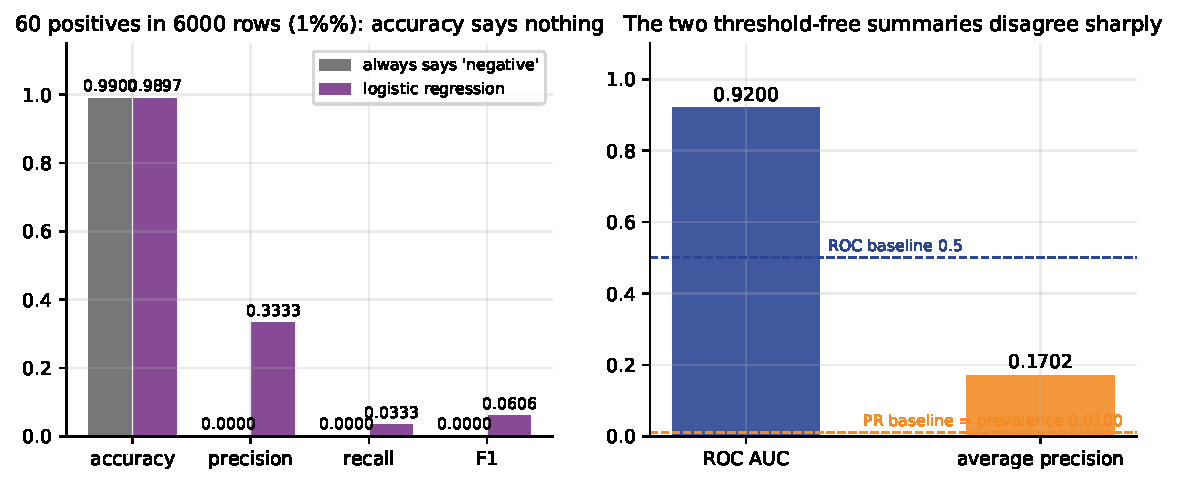
\includegraphics[width=0.88\textwidth]{l19-imbalance-accuracy.pdf}
  \end{center}
  \begin{center}\small
    Left: four metrics for the constant model and for logistic regression on
    the $99\!:\!1$ problem. \textbf{The accuracy bars are indistinguishable};
    precision and recall are not. Right: two threshold-free summaries of the
    \emph{same} logistic regression, each against its own baseline ---
    ROC AUC $0.9200$ against $0.5$, average precision $0.1702$ against the
    prevalence $0.0100$. They disagree, and we will see exactly why.
  \end{center}
\end{frame}

% =====================================================================
\section[Confusion]{The confusion matrix}
\label{sec:cm}

\begin{frame}[shrink=7]{Four boxes, and the naming rule}
  \begin{center}\small
  \begin{tabular}{@{}llll@{}}
    \toprule
     & predicted negative & predicted positive & row total\\
    \midrule
    actually negative & $\TN$ true negative  & $\FP$ false positive &
      $N = \FP + \TN$\\
    actually positive & $\FN$ false negative & $\TP$ true positive  &
      $P = \TP + \FN$\\
    \bottomrule
  \end{tabular}
  \end{center}
  \begin{exampleblock}{}
    \centering\small
    \textbf{The second word is what the model said; the first word is whether
    it was right.} A false positive is a row the model called positive and was
    wrong about.
  \end{exampleblock}
  \vspace{0.2em}
  \begin{center}\small
    \textbf{By hand.} Twenty people are screened. Ten have the disease (label
    $1$), ten do not. The model says ``disease'' for six of the ten who have
    it, and for two of the ten who do not.
  \end{center}
  \begin{center}\footnotesize
  \begin{tabular}{@{}lrrrrrrrrrr@{}}
    \toprule
    patient   & 1&2&3&4&5&6&7&8&9&10\\
    actual    & 1&1&1&1&1&1&1&1&1&1\\
    predicted & 1&1&1&1&1&1&0&0&0&0\\
    cell      & TP&TP&TP&TP&TP&TP&FN&FN&FN&FN\\
    \midrule
    patient   & 11&12&13&14&15&16&17&18&19&20\\
    actual    & 0&0&0&0&0&0&0&0&0&0\\
    predicted & 1&1&0&0&0&0&0&0&0&0\\
    cell      & FP&FP&TN&TN&TN&TN&TN&TN&TN&TN\\
    \bottomrule
  \end{tabular}
  \end{center}
  \begin{center}\small
    Count them: $\TP = 6$, $\FN = 4$, $\FP = 2$, $\TN = 8$, so $P = 10$ and
    $N = 10$.
  \end{center}
\end{frame}

\begin{frame}[shrink=9]{By hand: six metrics from four counts}
  \begin{columns}[T]
    \begin{column}{0.54\textwidth}
      \small
      \begin{align*}
        \text{accuracy} &= \frac{\TP + \TN}{P + N} = \frac{6+8}{20} = 0.7000\\
        \text{precision} &= \frac{\TP}{\TP + \FP} = \frac{6}{8} = 0.7500\\
        \text{recall} = \TPR &= \frac{\TP}{P} = \frac{6}{10} = 0.6000\\
        \text{specificity} &= \frac{\TN}{N} = \frac{8}{10} = 0.8000\\
        \FPR &= \frac{\FP}{N} = \frac{2}{10} = 0.2000\\
        F_1 &= \frac{2pr}{p + r} = \frac{2(0.75)(0.60)}{1.35}
          = \frac{0.9}{1.35} = 0.6667
      \end{align*}
    \end{column}
    \begin{column}{0.44\textwidth}
      \begin{block}{Six numbers, one source}
        \footnotesize Every metric in this lecture is a ratio of two of
        $\{\TP, \FP, \FN, \TN\}$. Nothing else is going on. Learn the four
        counts and you can rebuild the rest under examination conditions.
      \end{block}
      \begin{alertblock}{Two habits}
        \footnotesize \textbf{(1)} Write $P$ and $N$ down first --- most
        arithmetic errors are a wrong denominator.\\[0.3em]
        \textbf{(2)} $\FPR$ and specificity always sum to $1$. Compute one,
        subtract for the other, and you have a free check.
      \end{alertblock}
    \end{column}
  \end{columns}
\end{frame}

\begin{frame}[fragile,shrink=8]{The same twenty rows, in code}
\begin{lstlisting}
y_true = np.array([1]*10 + [0]*10)
y_pred = np.array([1]*6 + [0]*4 + [1]*2 + [0]*8)
print(confusion_matrix(y_true, y_pred))
print(classification_report(y_true, y_pred, digits=4,
      target_names=["healthy (0)", "disease (1)"]))
\end{lstlisting}
\begin{outblk}
confusion_matrix(y_true, y_pred) =
[[8 2]
 [4 6]]
rows = actual, cols = predicted, label order [0, 1]
so cm[1,1]=TP=6  cm[0,1]=FP=2  cm[1,0]=FN=4  cm[0,0]=TN=8

              precision    recall  f1-score   support

 healthy (0)     0.6667    0.8000    0.7273        10
 disease (1)     0.7500    0.6000    0.6667        10

    accuracy                         0.7000        20
   macro avg     0.7083    0.7000    0.6970        20
weighted avg     0.7083    0.7000    0.6970        20
\end{outblk}
\onslide<2->
\begin{alertblock}{The layout that catches everybody}
  \footnotesize \texttt{confusion\_matrix} puts \textbf{actual on the rows,
  predicted on the columns}, labels in sorted order --- so the top-left cell
  is $\TN$ and the bottom-right is $\TP$. That is the \emph{transpose} of Han,
  Kamber and Pei \S8.5.1 and of most textbook diagrams. Print it and check one
  cell against a count you did yourself.
\end{alertblock}
\end{frame}

\begin{frame}[shrink=9]{Drawn: four counts, six rates}
  \begin{center}
    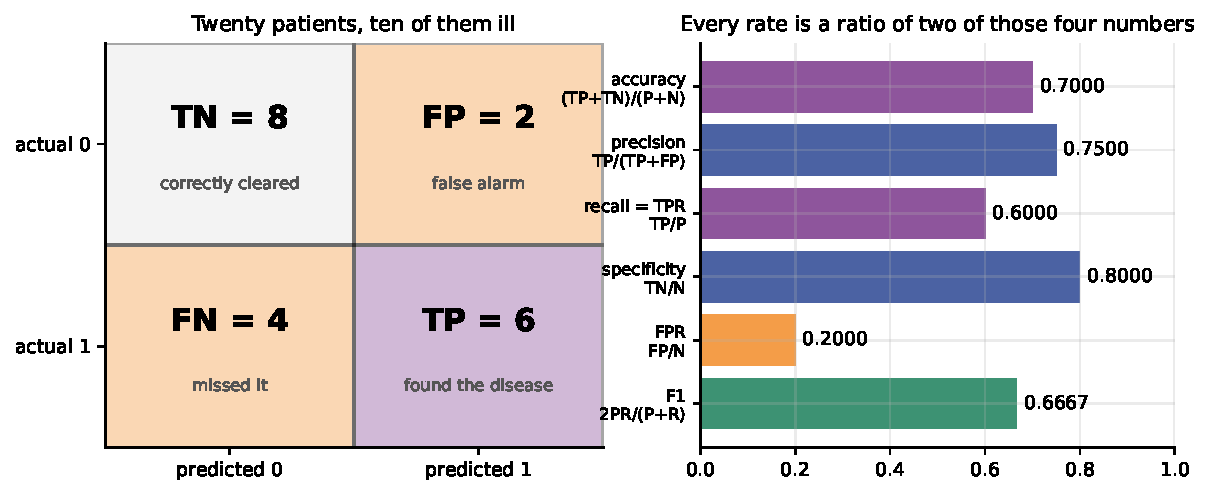
\includegraphics[width=0.80\textwidth]{l19-confusion-matrix.pdf}
  \end{center}
  \begin{center}\small
  \begin{tabular}{@{}llll@{}}
    \toprule
    name & formula & denominator is & answers\\
    \midrule
    recall / sensitivity / $\TPR$ & $\TP/P$ & the actual positives &
      of the ill, how many did we find?\\
    specificity / TNR & $\TN/N$ & the actual negatives &
      of the well, how many did we clear?\\
    $\FPR$ & $\FP/N$ & the actual negatives &
      of the well, how many did we alarm?\\
    precision / PPV & $\TP/(\TP{+}\FP)$ & the \emph{predicted} positives &
      of our alarms, how many were real?\\
    \bottomrule
  \end{tabular}
  \end{center}
\end{frame}

\begin{frame}[shrink=10]{Precision is the odd one out}
  \begin{exampleblock}{}
    \centering\small
    Recall and $\FPR$ divide by a \emph{class size}, so they do not move when
    you change how many negatives you happened to collect. Precision divides
    by $\TP + \FP$, which the \textbf{prevalence} controls. \textbf{That one
    difference is why the ROC curve is blind to imbalance and the
    precision--recall curve is not.}
  \end{exampleblock}
  \vspace{0.2em}
  \begin{columns}[T]
    \begin{column}{0.48\textwidth}
      \begin{block}{Why the harmonic mean}
        \small $F_1$ combines precision and recall, and the harmonic mean is
        \emph{dominated by the smaller of the two}. A model that fires almost
        never but is always right when it does: $p = 1.0$, $r = 0.02$.
        Arithmetic mean $0.51$; harmonic mean $\mathbf{0.0392}$. The first
        flatters, the second reports.
      \end{block}
    \end{column}
    \begin{column}{0.48\textwidth}
      \begin{alertblock}{$F_\beta$, when a miss and an alarm differ}
        \small
        \[
          F_\beta = (1 + \beta^2)\,
            \frac{p \times r}{\beta^2 p + r}
        \]
        $\beta = 1$ is $F_1$. $F_2$ weights recall four times as heavily and
        is the choice when a miss hurts more. \textbf{Choosing $\beta$ is a
        business decision that has walked into the arithmetic.}
      \end{alertblock}
    \end{column}
  \end{columns}
\end{frame}

% =====================================================================
\section[Scores]{Scores, not labels}
\label{sec:scores}

\begin{frame}[shrink=7]{\texttt{predict} applies a threshold you never chose}
  \begin{center}\small
  \begin{tabular}{@{}lll@{}}
    \toprule
    model & score & default rule\\
    \midrule
    \texttt{LogisticRegression}     & \texttt{predict\_proba(X)[:, 1]} &
      positive if $\ge 0.5$\\
    \texttt{RandomForestClassifier} & \texttt{predict\_proba(X)[:, 1]} &
      positive if $\ge 0.5$\\
    \texttt{GaussianNB}             & \texttt{predict\_proba(X)[:, 1]} &
      positive if $\ge 0.5$\\
    \texttt{KNeighborsClassifier}   & fraction of the $k$ neighbours &
      positive if $\ge 0.5$\\
    \texttt{SVC}                    & \texttt{decision\_function(X)} &
      positive if $\ge 0$\\
    \texttt{MLPClassifier}          & \texttt{predict\_proba(X)[:, 1]} &
      positive if $\ge 0.5$\\
    \bottomrule
  \end{tabular}
  \end{center}
  \vspace{0.2em}
  \begin{alertblock}{}
    \centering\small
    Everything in the previous section describes \emph{one} confusion matrix,
    and a confusion matrix needs hard labels. \textbf{But a classifier does
    not naturally produce hard labels.} It produces a score, and
    \texttt{predict} silently compares it with $0.5$ --- a number nobody in
    the room chose.
  \end{alertblock}
\end{frame}

\begin{frame}[fragile,shrink=6]{The model we use for the rest of the lecture}
Deliberately \emph{imperfect}: logistic regression on three of the thirty
\texttt{breast\_cancer} columns, so that the choice of threshold has visible
consequences.
\begin{lstlisting}
COLS = [0, 1, 4]     # mean radius, mean texture, mean smoothness
Xb_tr, Xb_te, yb_tr, yb_te = train_test_split(
    Xb[:, COLS], yb, test_size=0.3, stratify=yb, random_state=0)
clf = make_pipeline(StandardScaler(),
                    LogisticRegression(max_iter=5000)).fit(Xb_tr, yb_tr)
sb = clf.predict_proba(Xb_te)[:, 1]
\end{lstlisting}
\begin{outblk}
features used: ['mean radius', 'mean texture', 'mean smoothness']
held-out rows 171   benign (positive) 107   malignant 64
ROC AUC 0.9661   accuracy at 0.5 0.9064
for comparison, the same split with all 30 features: ROC AUC 0.9956
we use the three-feature model from here on: a near-perfect model
makes every threshold look equally good, which teaches nothing.
\end{outblk}
\onslide<2->
\begin{center}\small
  Note which class is positive: in \texttt{load\_breast\_cancer} the label $1$
  is \textbf{benign}, the harmless one. \textbf{Every metric today is
  asymmetric between the classes, so decide which class is positive and say
  so out loud before you compute anything.}
\end{center}
\end{frame}

\begin{frame}[fragile,shrink=8]{One set of scores, seven confusion matrices}
\begin{lstlisting}
for t in [0.05, 0.20, 0.35, 0.50, 0.65, 0.80, 0.95]:
    p = (sb >= t).astype(int)
    print(t, accuracy_score(yb_te, p), precision_score(yb_te, p),
          recall_score(yb_te, p), f1_score(yb_te, p))
print("ROC AUC", roc_auc_score(yb_te, sb))
\end{lstlisting}
\begin{outblk}
one set of scores, one AUC, many thresholds
threshold  TP  FP  FN  TN  accuracy  precision  recall     F1
   0.05    107  28   0  36    0.8363     0.7926  1.0000  0.8843
   0.20    107  19   0  45    0.8889     0.8492  1.0000  0.9185
   0.35    106  13   1  51    0.9181     0.8908  0.9907  0.9381
   0.50    100   9   7  55    0.9064     0.9174  0.9346  0.9259
   0.65     94   4  13  60    0.9006     0.9592  0.8785  0.9171
   0.80     86   4  21  60    0.8538     0.9556  0.8037  0.8731
   0.95     58   0  49  64    0.7135     1.0000  0.5421  0.7030
ROC AUC, for every row above:  0.9661
AUC is a property of the scores. The threshold is a separate decision.
\end{outblk}
\onslide<2->
\begin{alertblock}{Accuracy $0.7135$ to $0.9181$, from one fitted model}
  \footnotesize Lower the threshold and recall climbs to $1.0000$ while
  precision falls to $0.7926$; raise it and the reverse. There is no threshold
  at which both improve, because raising it can only move rows from
  ``predicted positive'' to ``predicted negative''. \textbf{Quoting a single
  accuracy is quoting a model \emph{and} an unstated threshold as if they were
  one thing.}
\end{alertblock}
\end{frame}

\begin{frame}[shrink=8]{Drawn: the whole threshold sweep, two ways}
  \begin{center}
    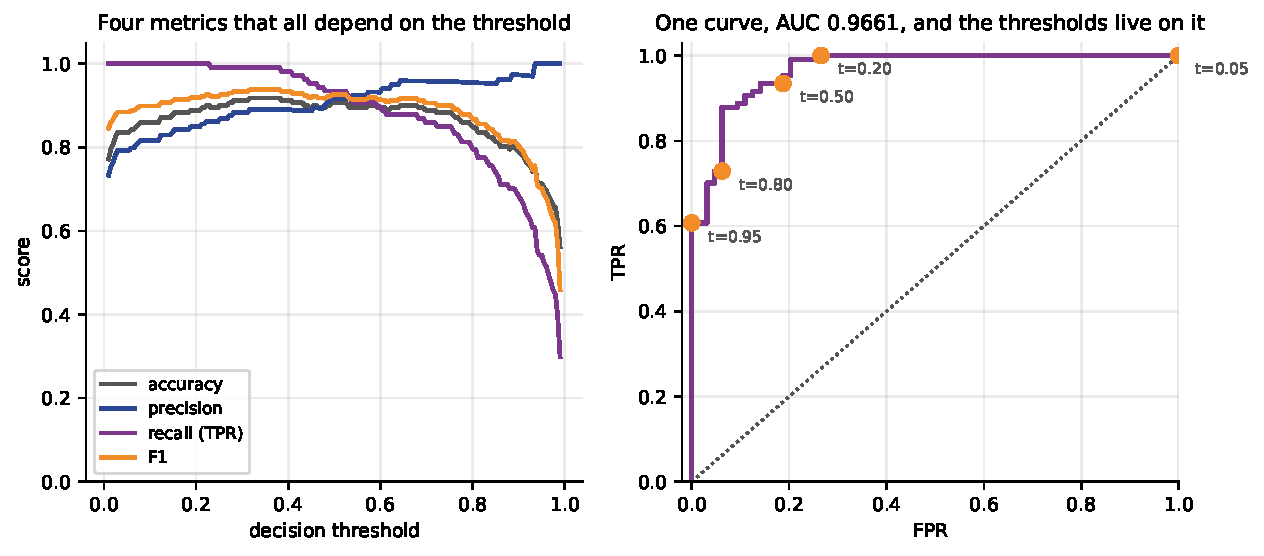
\includegraphics[width=0.88\textwidth]{l19-threshold-sweep.pdf}
  \end{center}
  \begin{center}\small
    Left: the four threshold-dependent metrics as continuous functions of the
    threshold. Right: \textbf{the same information as a single curve}. Each
    labelled point is one row of the table you just saw; the curve is every
    threshold at once. \textbf{That curve is the object this lecture is
    about}, and we are going to build it by hand before we let a library draw
    it.
  \end{center}
\end{frame}

% =====================================================================
\section[ROC]{Building an ROC curve by hand}
\label{sec:rochand}

\begin{frame}[shrink=7]{Ten scored examples, by hand}
Five positives, five negatives, each with a score between $0$ and $1$. Sorted
by score, highest first.
  \begin{center}\small
  \begin{tabular}{@{}rrrrrrrrrrr@{}}
    \toprule
    rank  & 1 & 2 & 3 & 4 & 5 & 6 & 7 & 8 & 9 & 10\\
    label & POS & POS & \emph{neg} & POS & POS & \emph{neg} & \emph{neg} &
            POS & \emph{neg} & \emph{neg}\\
    score & $0.95$ & $0.90$ & $0.85$ & $0.75$ & $0.60$ & $0.55$ & $0.45$ &
            $0.35$ & $0.25$ & $0.10$\\
    \bottomrule
  \end{tabular}
  \end{center}
  \vspace{0.2em}
  \begin{columns}[T]
    \begin{column}{0.48\textwidth}
      \begin{block}{$P = 5$, $N = 5$}
        \small The model is not perfect --- a negative sits at rank $3$, above
        two positives --- but it is clearly better than nothing. Those two
        facts are what the curve will show.
      \end{block}
    \end{column}
    \begin{column}{0.48\textwidth}
      \begin{alertblock}{Get a pen out now}
        \small We are going to sweep the threshold down this list and compute
        $(\FPR, \TPR)$ at every step. \textbf{Do it with me.} The library will
        not appear for four frames, and when it does its output must match
        yours row for row.
      \end{alertblock}
    \end{column}
  \end{columns}
\end{frame}

\begin{frame}[shrink=6]{The recipe: up for POS, right for neg}
  \begin{exampleblock}{}
    \centering\small
    Start with the threshold \emph{above every score}: nothing is predicted
    positive, $\TP = \FP = 0$, and the point is $(0, 0)$. Now lower the
    threshold to each score in turn.
  \end{exampleblock}
  \vspace{0.2em}
  \begin{columns}[T]
    \begin{column}{0.48\textwidth}
      \begin{block}{Cross a POSITIVE}
        \small One row moves from $\FN$ to $\TP$. So $\TPR$ rises by
        $1/P = 0.2$ and $\FPR$ does not move.\\[0.3em]
        \centering\textbf{A step UP.}
      \end{block}
    \end{column}
    \begin{column}{0.48\textwidth}
      \begin{block}{Cross a NEGATIVE}
        \small One row moves from $\TN$ to $\FP$. So $\FPR$ rises by
        $1/N = 0.2$ and $\TPR$ does not move.\\[0.3em]
        \centering\textbf{A step RIGHT.}
      \end{block}
    \end{column}
  \end{columns}
  \vspace{0.3em}
  \begin{alertblock}{}
    \centering\small
    Ten rows, ten steps, eleven points --- and the two endpoints are
    guaranteed: $(0,0)$ when nothing is called positive, $(1,1)$ when
    everything is. \textbf{Every ROC curve you will ever see runs between
    those two corners.}
  \end{alertblock}
\end{frame}

\begin{frame}[shrink=6]{By hand: the first five steps, one at a time}
The sorted labels are \textbf{POS, POS, \emph{neg}, POS, POS, \dots}
  \begin{itemize}\small
    \item<1-> \textbf{Threshold above everything.} $\TP = 0$, $\FP = 0$,
      $\FN = 5$, $\TN = 5$. Point $(0.0,\, 0.0)$. Start here, always.
    \item<2-> \textbf{$t = 0.95$, a POSITIVE.} $\TP = 1$, $\FP = 0$.
      $\FPR = 0/5 = 0.0$, $\TPR = 1/5 = 0.2$. Point $(0.0,\, 0.2)$ ---
      \emph{up}.
    \item<3-> \textbf{$t = 0.90$, a POSITIVE.} $\TP = 2$, $\FP = 0$.
      Point $(0.0,\, 0.4)$ --- \emph{up} again. We are climbing the left-hand
      edge, which is exactly what a good model does.
    \item<4-> \textbf{$t = 0.85$, a \emph{negative}.} $\TP = 2$, $\FP = 1$.
      $\FPR = 1/5 = 0.2$, $\TPR$ unchanged at $0.4$. Point $(0.2,\, 0.4)$ ---
      \emph{right}. \textbf{This is the model's one mistake, and it is the
      only reason the area will not be $1$.}
    \item<5-> \textbf{$t = 0.75$, a POSITIVE.} $\TP = 3$, $\FP = 1$.
      Point $(0.2,\, 0.6)$ --- up.
    \item<6-> \textbf{Nothing has been fitted, smoothed or estimated.} This is
      bookkeeping on a sorted list, and you could finish it in the margin of a
      question paper.
  \end{itemize}
\end{frame}

\begin{frame}[shrink=8]{By hand: the whole sweep, eleven points}
  \begin{columns}[T]
    \begin{column}{0.58\textwidth}
      \begin{center}\footnotesize
      \begin{tabular}{@{}lrrrrrr@{}}
        \toprule
        threshold & $\TP$ & $\FP$ & $\FN$ & $\TN$ & $\FPR$ & $\TPR$\\
        \midrule
        (nothing) & 0 & 0 & 5 & 5 & $0.0$ & $0.0$\\
        $0.95$ (POS) & 1 & 0 & 4 & 5 & $0.0$ & $0.2$\\
        $0.90$ (POS) & 2 & 0 & 3 & 5 & $0.0$ & $0.4$\\
        $0.85$ (neg) & 2 & 1 & 3 & 4 & $0.2$ & $0.4$\\
        $0.75$ (POS) & 3 & 1 & 2 & 4 & $0.2$ & $0.6$\\
        $0.60$ (POS) & 4 & 1 & 1 & 4 & $0.2$ & $0.8$\\
        $0.55$ (neg) & 4 & 2 & 1 & 3 & $0.4$ & $0.8$\\
        $0.45$ (neg) & 4 & 3 & 1 & 2 & $0.6$ & $0.8$\\
        $0.35$ (POS) & 5 & 3 & 0 & 2 & $0.6$ & $1.0$\\
        $0.25$ (neg) & 5 & 4 & 0 & 1 & $0.8$ & $1.0$\\
        $0.10$ (neg) & 5 & 5 & 0 & 0 & $1.0$ & $1.0$\\
        \bottomrule
      \end{tabular}
      \end{center}
    \end{column}
    \begin{column}{0.40\textwidth}
      \begin{exampleblock}{That table \emph{is} the ROC curve}
        \footnotesize Plot the eleven $(\FPR, \TPR)$ pairs, join them with
        horizontal and vertical segments, and the staircase is finished.
      \end{exampleblock}
      \begin{block}{Read the pattern in the label column}
        \footnotesize POS POS \emph{neg} POS POS \emph{neg} \emph{neg} POS
        \emph{neg} \emph{neg} becomes\\
        up up \textbf{right} up up \textbf{right} \textbf{right} up
        \textbf{right} \textbf{right}.\\[0.3em]
        \textbf{The curve depends only on the \emph{order} of the scores, not
        on their values} --- so any monotone rescaling leaves it untouched.
      \end{block}
    \end{column}
  \end{columns}
\end{frame}

\begin{frame}[fragile,shrink=8]{Predict first \#2}
\begin{lstlisting}
y10 = np.array([1, 1, 0, 1, 1, 0, 0, 1, 0, 0])
s10 = np.array([0.95, 0.90, 0.85, 0.75, 0.60, 0.55, 0.45, 0.35, 0.25, 0.10])
fpr, tpr, thr = roc_curve(y10, s10, drop_intermediate=False)
\end{lstlisting}
\begin{center}
  \textbf{How many rows will this print, what will the first threshold be, and
  will any row disagree with your table?}
\end{center}
\onslide<2->
\begin{outblk}
sklearn roc_curve(y, s, drop_intermediate=False)
 threshold      FPR     TPR
       inf  0.0000  0.0000
      0.95  0.0000  0.2000
      0.90  0.0000  0.4000
      0.85  0.2000  0.4000
      0.75  0.2000  0.6000
      0.60  0.2000  0.8000
      0.55  0.4000  0.8000
      0.45  0.6000  0.8000
      0.35  0.6000  1.0000
      0.25  0.8000  1.0000
      0.10  1.0000  1.0000
the first threshold is np.inf: the 'predict nothing' corner (0,0).
every other row matches the hand sweep exactly.
\end{outblk}
\onslide<3->
\begin{outblk}
with the default drop_intermediate=True sklearn keeps only the corners:
  8 points instead of 11, same curve, same area 0.8000
\end{outblk}
\end{frame}

\begin{frame}[shrink=8]{Drawn: your staircase, and how to read one}
  \begin{center}
    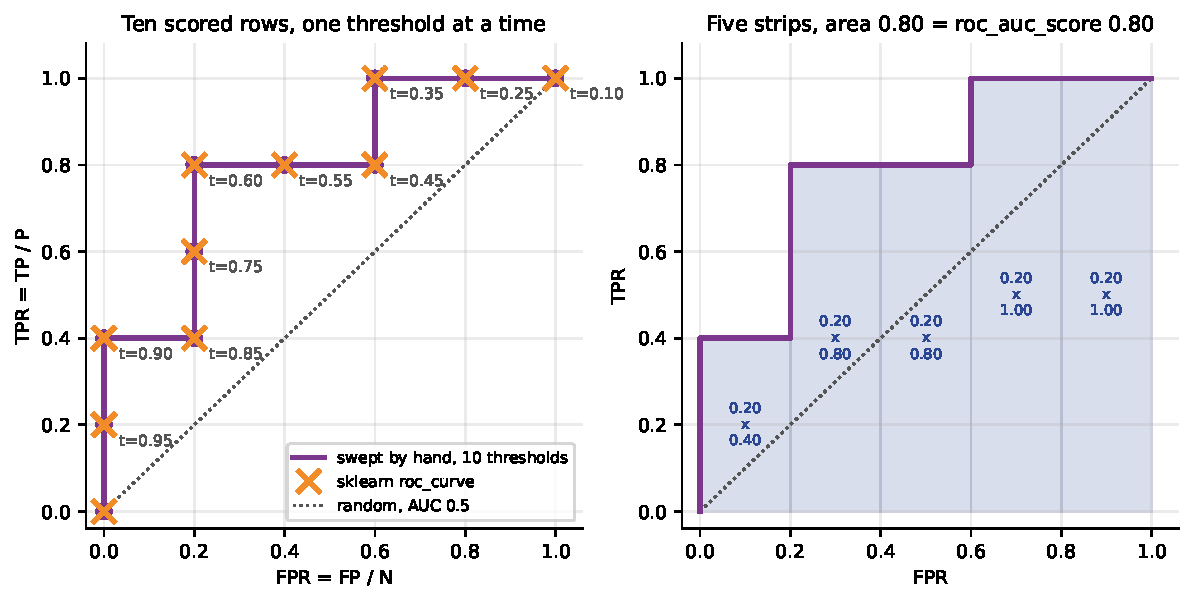
\includegraphics[width=0.60\textwidth]{l19-roc-by-hand.pdf}
  \end{center}
  \begin{center}\small
    Left: your staircase with its threshold labels, and \texttt{roc\_curve}'s
    crosses on top. \textbf{The largest disagreement is $0.00$.} Right: the
    five strips whose areas we are about to add up.
  \end{center}
  \begin{center}\footnotesize
    \textbf{Four things to look for.} $(0,1)$ is the perfect classifier, so
    closer is better; the diagonal is a score with no information;
    \emph{steepness at the left} is what matters in practice; and a dip below
    the diagonal means the score is anti-correlated over that band.
  \end{center}
\end{frame}

% =====================================================================
\section[AUC]{AUC, computed two ways}
\label{sec:auc}

\begin{frame}[fragile,shrink=8]{By hand: the area, as five trapezoids}
The curve is piecewise linear, so the trapezoidal rule is \emph{exact}. Cut the
region into vertical strips, one per horizontal move; each strip is
$0.2$ wide and as tall as the $\TPR$ during that move.
  \begin{columns}[T]
    \begin{column}{0.44\textwidth}
      \begin{center}\small
      \begin{tabular}{@{}rrrrr@{}}
        \toprule
        from & to & width & $\TPR$ & area\\
        \midrule
        $0.0$ & $0.2$ & $0.2$ & $0.4$ & $0.08$\\
        $0.2$ & $0.4$ & $0.2$ & $0.8$ & $0.16$\\
        $0.4$ & $0.6$ & $0.2$ & $0.8$ & $0.16$\\
        $0.6$ & $0.8$ & $0.2$ & $1.0$ & $0.20$\\
        $0.8$ & $1.0$ & $0.2$ & $1.0$ & $0.20$\\
        \midrule
        \multicolumn{4}{r}{total} & $\mathbf{0.80}$\\
        \bottomrule
      \end{tabular}
      \end{center}
    \end{column}
    \begin{column}{0.54\textwidth}
\begin{outblk}
  from      to     width  height (TPR)   strip
  0.00    0.20      0.20        0.40       0.0800
  0.20    0.40      0.20        0.80       0.1600
  0.40    0.60      0.20        0.80       0.1600
  0.60    0.80      0.20        1.00       0.2000
  0.80    1.00      0.20        1.00       0.2000
trapezoidal area                                 0.8000
sklearn auc(fpr, tpr)                            0.8000
sklearn roc_auc_score(y, s)                      0.8000
\end{outblk}
    \end{column}
  \end{columns}
\onslide<2->
\begin{center}\small
  \texttt{auc(fpr, tpr)} integrates the curve you were given;
  \texttt{roc\_auc\_score(y, s)} builds the curve itself and integrates that.
  \textbf{Same $0.8000$, and the hand sum $0.08 + 0.16 + 0.16 + 0.20 + 0.20$
  is the same arithmetic.}
\end{center}
\end{frame}

\begin{frame}[shrink=7]{By hand: the same number, without a drawing}
There are $P \times N = 5 \times 5 = 25$ ways to pick one positive and one
negative. Count the pairs the model ordered \emph{correctly}.
  \begin{columns}[T]
    \begin{column}{0.46\textwidth}
      \begin{center}\small
      \begin{tabular}{@{}lr@{}}
        \toprule
        negative scored & positives above it\\
        \midrule
        $0.85$ & $2$\\
        $0.55$ & $4$\\
        $0.45$ & $4$\\
        $0.25$ & $5$\\
        $0.10$ & $5$\\
        \midrule
        total & $\mathbf{20}$ of $25$\\
        \bottomrule
      \end{tabular}
      \end{center}
      \begin{center}\footnotesize
        Only $0.95$ and $0.90$ beat the negative at $0.85$;\\
        every positive beats the two lowest negatives.
      \end{center}
    \end{column}
    \begin{column}{0.50\textwidth}
      \begin{exampleblock}{$20/25 = \mathbf{0.80}$}
        \small The same number the trapezoids gave. \textbf{It is not a
        coincidence and it is not an approximation.} It is an identity:
        \[
          \mathrm{AUC} = \Pr\!\big(s(X^{+}) > s(X^{-})\big)
            + \tfrac{1}{2}\Pr\!\big(s(X^{+}) = s(X^{-})\big)
        \]
        with $X^{+}, X^{-}$ drawn independently from the positives and the
        negatives. \textbf{Ties count a half} --- which is exactly what the
        diagonal segments of a staircase contribute.
      \end{exampleblock}
    \end{column}
  \end{columns}
\end{frame}

\begin{frame}[fragile,shrink=8]{The pair count, and what it turns out to be}
\begin{outblk}
for each negative: how many positives outrank it?
  negative scored 0.85  ->  2 of the 5 positives above it
  negative scored 0.55  ->  4 of the 5 positives above it
  negative scored 0.45  ->  4 of the 5 positives above it
  negative scored 0.25  ->  5 of the 5 positives above it
  negative scored 0.10  ->  5 of the 5 positives above it
concordant pairs 20   ties 0   total pairs 25
P(random positive outranks random negative) = 20/25 = 0.8000
roc_auc_score                               = 0.8000
\end{outblk}
\onslide<2->
\begin{lstlisting}
U = stats.mannwhitneyu(pos, neg, alternative="greater").statistic
print(U, U / (len(pos) * len(neg)), roc_auc_score(y10, s10))
\end{lstlisting}
\begin{outblk}
Mann-Whitney U statistic  20.0
U / (n_pos * n_neg)       0.8000
roc_auc_score             0.8000
AUC and the Mann-Whitney U statistic are the same quantity, rescaled.
\end{outblk}
\onslide<3->
\begin{center}\small
  So the AUC of a set of scores and the rank-sum test of ``do the positives
  score higher than the negatives?'' are \textbf{the same computation}, and
  Hanley and McNeil's $1982$ paper is where that was first written down.
\end{center}
\end{frame}

\begin{frame}[shrink=8]{Drawn: twenty-five pairs, and a million}
  \begin{center}
    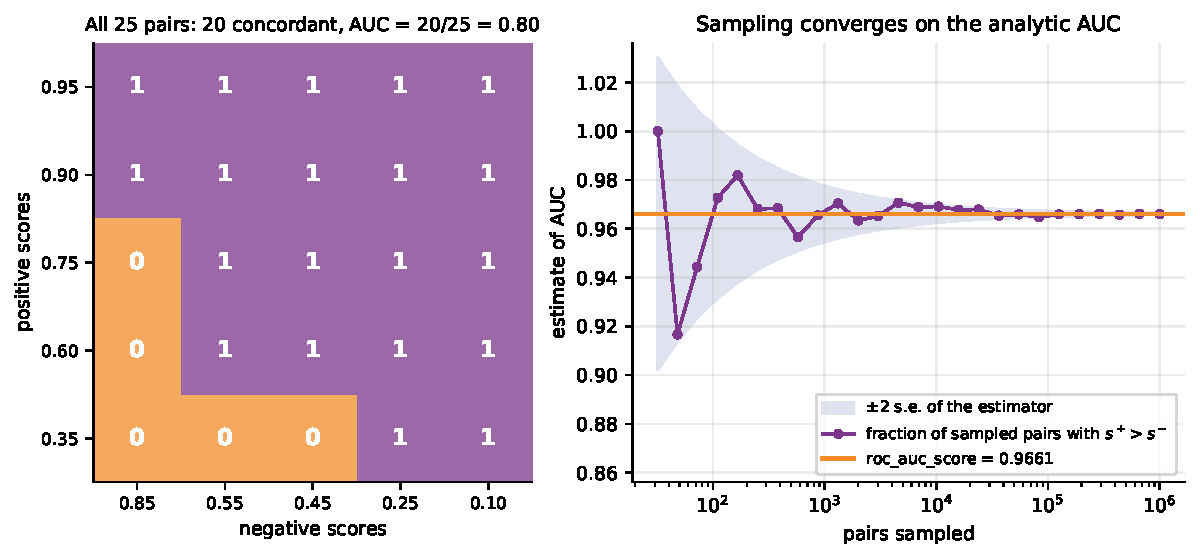
\includegraphics[width=0.88\textwidth]{l19-auc-pairs.pdf}
  \end{center}
  \begin{center}\small
    Left: all $25$ positive--negative pairs from the ten hand rows; a mark
    means the model ordered that pair correctly. \textbf{Twenty of
    twenty-five, AUC $0.80$} --- you can literally count the picture. Right:
    the sampled estimate on \texttt{breast\_cancer} converging on the analytic
    $0.966121$, inside the $\pm 2$ standard-error band of a Bernoulli
    proportion --- $100$ pairs give $0.980000$, ten million give $0.966230$,
    and counting all $\mathbf{6848}$ pairs exactly reproduces
    \texttt{roc\_auc\_score} to a difference of
    $\mathbf{0.00\mathrm{e}{+}00}$. \textbf{AUC is not \emph{like} that
    probability; it is that probability.}
  \end{center}
\end{frame}

\begin{frame}[fragile,shrink=6]{Predict first \#3}
\begin{lstlisting}
rng = np.random.default_rng(0)       # the one seed for this lecture
yr, sr = rng.integers(0, 2, 2000), rng.random(2000)
print(roc_auc_score(yr, sr))
\end{lstlisting}
Two thousand coin-flip labels, two thousand uniform random scores. There is no
model here at all.
\begin{center}
  \textbf{What AUC comes out --- and, harder, how far from it can one run
  stray?}
\end{center}
\onslide<2->
\begin{outblk}
2000 coin-flip labels, 2000 uniform random scores
  roc_auc_score  0.5023
  accuracy at threshold 0.5  0.5090
  200 repetitions: mean 0.4994  sd 0.0136  min 0.4645  max 0.5342
  the diagonal is not a curve you draw, it is the answer you get
  when the score carries no information about the label.
\end{outblk}
\onslide<3->
\begin{center}\small
  That spread is the useful part. \textbf{On $2000$ rows an AUC of $0.53$ is
  not evidence of anything} --- the noise runs to $0.5342$ on its own.
\end{center}
\end{frame}

\begin{frame}[fragile,shrink=8]{An AUC below $0.5$ is a different animal}
  \begin{columns}[T]
    \begin{column}{0.56\textwidth}
\begin{lstlisting}
print(roc_auc_score(yb_te,  sb),
      roc_auc_score(yb_te, -sb),
      roc_auc_score(1 - yb_te, sb))
\end{lstlisting}
\begin{outblk}
the fitted breast_cancer model              AUC 0.9661
the same model with its scores negated      AUC 0.0339
the same model with the labels swapped      AUC 0.0339
1 - AUC                                         0.0339
An AUC of 0.0339 is not a bad model. It is this model wired backwards:
flip the sign of the score and you get 0.9661 back.
\end{outblk}
    \end{column}
    \begin{column}{0.42\textwidth}
      \begin{center}
        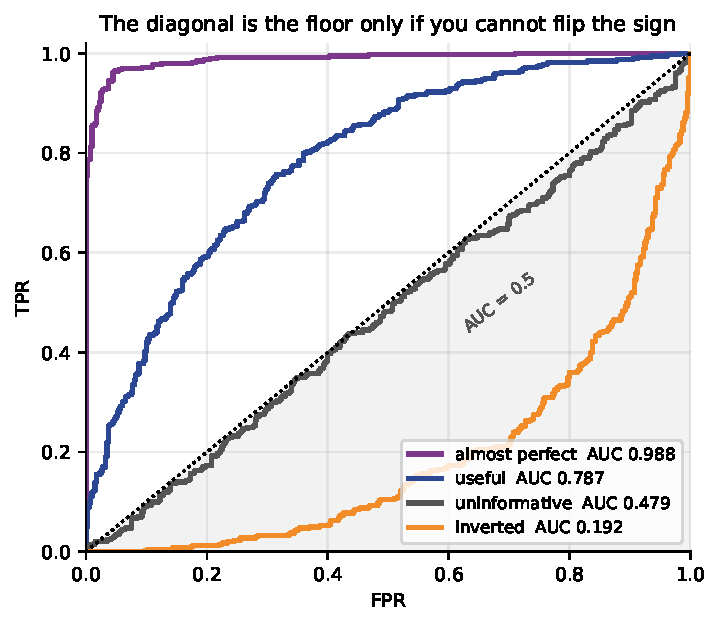
\includegraphics[width=\textwidth]{l19-roc-families.pdf}
      \end{center}
    \end{column}
  \end{columns}
\onslide<2->
\begin{alertblock}{$\mathrm{AUC}(-s) = 1 - \mathrm{AUC}(s)$, exactly}
  \footnotesize Negating the score reverses every pairwise comparison, so
  $0.5$ --- not $0$ --- is the floor for a model you are allowed to relabel.
  \textbf{An AUC well below $0.5$ almost always means you passed the wrong
  column of \texttt{predict\_proba}, or defined the positive class one way and
  scored it the other.} In the figure the ``inverted'' curve at $0.192$
  becomes $0.808$ the moment you flip a sign.
\end{alertblock}
\end{frame}

\begin{frame}[fragile,shrink=8]{The two invariances}
\textbf{Threshold.} Look again at the sweep: the threshold is a \emph{row
label}, never an input. Accuracy moved $0.7135 \to 0.9181$ across seven
thresholds while AUC sat at $0.9661$ throughout.\\[0.2em]
\textbf{Class balance.} Keep every positive, throw negatives away at random.
$\TPR$ lives inside the positives and $\FPR$ inside the negatives.
\begin{outblk}
same model, same scores; only the negatives are subsampled
 negatives kept  prevalence   ROC AUC   avg precision
           5940      0.0100    0.9200       0.1702
           2000      0.0291    0.9197       0.3380
            500      0.1071    0.9172       0.6699
            120      0.3333    0.9243       0.8839
             60      0.5000    0.9158       0.9202
ROC AUC is invariant to class balance. Average precision is not:
  it rose from 0.1702 to 0.9202 -- a factor of 5.4 -- without the model
  changing at all.
\end{outblk}
\onslide<2->
\begin{center}\small
  ROC AUC moved $0.0092$ over a \textbf{fiftyfold} change in prevalence ---
  sampling noise. Average precision moved by a factor of $\mathbf{5.4}$.
  \textbf{One fixed set of scores. Nothing about the model changed.} That
  single table is the whole of the next section.
\end{center}
\end{frame}

% =====================================================================
\section[ROC/PR]{ROC against precision--recall}
\label{sec:rocpr}

\begin{frame}[fragile,shrink=9]{Where ROC flatters: the $99\!:\!1$ problem
again}
\begin{outblk}
the 99:1 problem, logistic regression, 6000 held-out rows
  prevalence            0.0100  (60 positives, 5940 negatives)
  ROC AUC               0.9200   (baseline 0.5000)
  average precision     0.1702   (baseline = prevalence = 0.0100)

  recall   precision   threshold    TP    FP
   0.10      0.2400      0.3634      6    19
   0.30      0.2647      0.2004     18    50
   0.50      0.1648      0.0719     30   152
   0.70      0.0955      0.0275     42   398
   0.90      0.0439      0.0069     54  1177
   1.00      0.0100      0.0000     60  5940

  ROC reads: at TPR 0.9000 the FPR is only 0.1946 -- encouraging.
  PR reads:  0.1946 x 5940 = 1156 false alarms for 54 true ones,
             precision 0.0446. One alert in 22 is real.
\end{outblk}
\onslide<2->
\begin{alertblock}{Both readings are true. Only one is the client's question}
  \footnotesize AUC $0.9200$ \emph{is} a strong model in the precise sense AUC
  measures: pick a random positive and a random negative and it orders them
  correctly $92\%$ of the time. But to catch $90\%$ of the positives you must
  accept \textbf{$1156$ false alarms alongside $54$ real ones}. The $\FPR$ of
  $0.1946$ that looked small on the ROC axis is $19.46\%$ of $5940$ negatives
  --- and $5940$ is a large number.
\end{alertblock}
\end{frame}

\begin{frame}[shrink=9]{Drawn: one model, two pictures, two verdicts}
  \begin{center}
    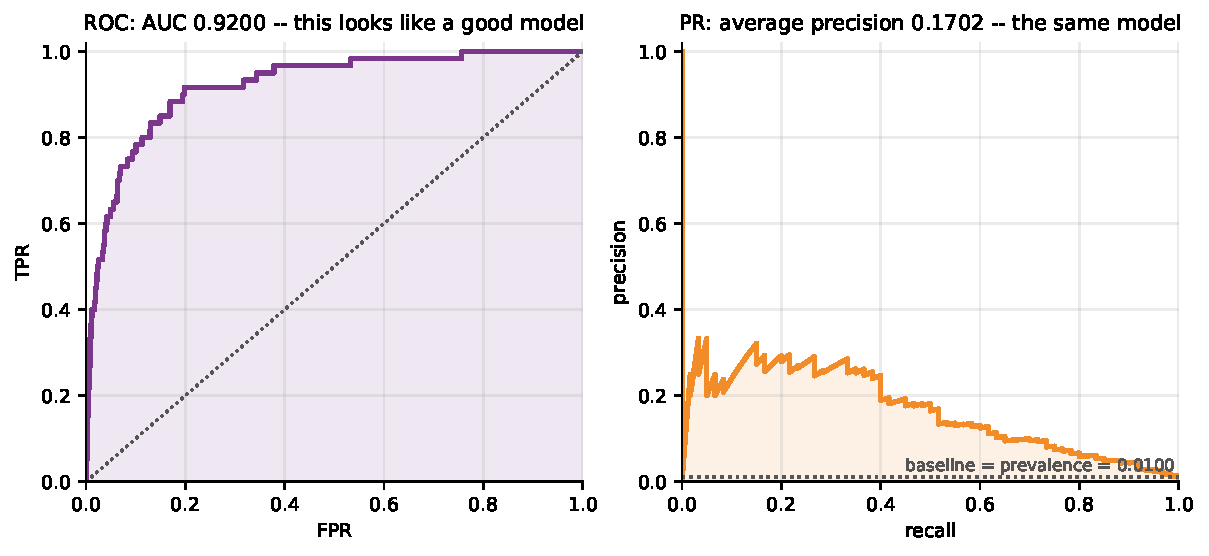
\includegraphics[width=0.80\textwidth]{l19-roc-vs-pr.pdf}
  \end{center}
  \begin{center}\small
  \begin{tabular}{@{}llll@{}}
    \toprule
     & axes & baseline of a useless model & moves with prevalence?\\
    \midrule
    ROC & $\TPR$ against $\FPR$ & the diagonal, AUC $= 0.5$ & no\\
    PR  & precision against recall & the horizontal line at the prevalence &
      \textbf{yes}\\
    \bottomrule
  \end{tabular}
  \end{center}
  \begin{center}\small
    \textbf{$\FPR$ divides by the number of negatives, which is huge when
    positives are rare, so a large absolute number of false alarms shows up as
    a small $\FPR$.} Precision divides by $\TP + \FP$ instead, and when $\FP$
    swamps $\TP$ it falls off a cliff.
  \end{center}
\end{frame}

\begin{frame}[shrink=9]{Drawn: five prevalences, one set of scores}
  \begin{center}
    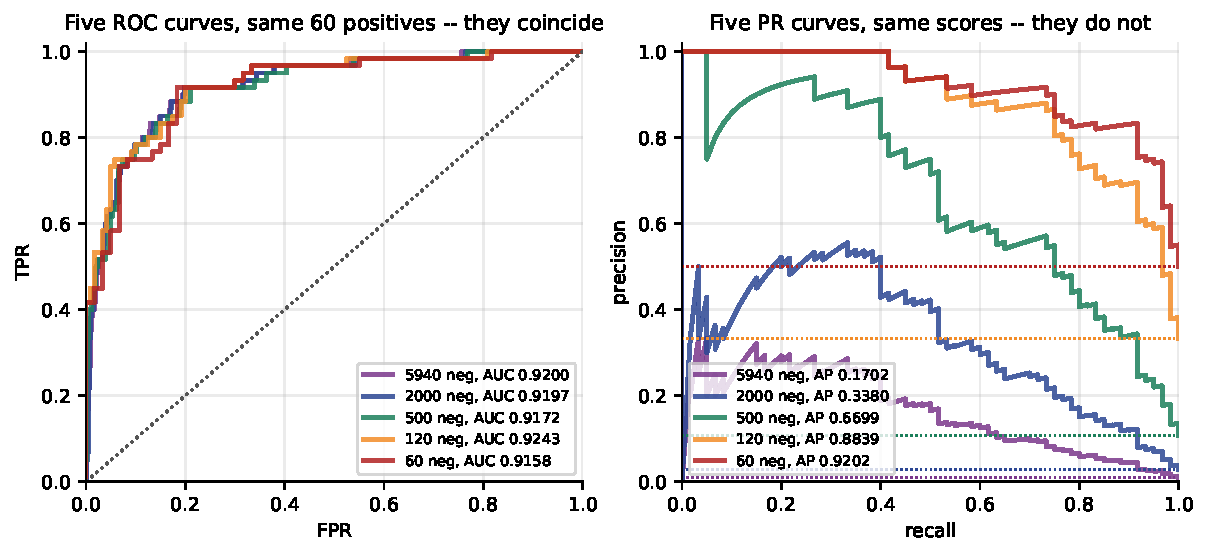
\includegraphics[width=0.80\textwidth]{l19-balance-invariance.pdf}
  \end{center}
  \begin{columns}[T]
    \begin{column}{0.48\textwidth}
      \begin{block}{Report \textbf{ROC AUC} when\dots}
        \footnotesize the classes are comparably common; or you want a summary
        that will not shift because next month's data has a different mix; or
        a false positive and a false negative cost about the same.
      \end{block}
    \end{column}
    \begin{column}{0.48\textwidth}
      \begin{alertblock}{Report \textbf{average precision} when\dots}
        \footnotesize positives are rare and somebody is going to \emph{act}
        on the alerts. Fraud review, medical triage, moderation --- a human
        has finite capacity, and precision is exactly the fraction of their
        time that is not wasted. \textbf{Always quote the prevalence beside
        it.}
      \end{alertblock}
    \end{column}
  \end{columns}
  \begin{center}\small
    And the invariance runs both ways: an AUC measured on a balanced subsample
    \emph{transfers} to the imbalanced population; \textbf{an average precision
    does not.} Final evaluation goes on data with the production prevalence.
  \end{center}
\end{frame}

% =====================================================================
\section[Threshold]{Choosing the threshold is a business decision}
\label{sec:threshold}

\begin{frame}[shrink=13]{$0.5$ is an assumption --- and Youden's $J$ by hand}
  \begin{exampleblock}{}
    \centering\small
    \texttt{predict} thresholds at $0.5$. That is optimal under exactly one
    condition: \textbf{a false positive and a false negative cost the same}.
  \end{exampleblock}
  \begin{columns}[T]
    \begin{column}{0.40\textwidth}
      \begin{center}\scriptsize
      \begin{tabular}{@{}rrrr@{}}
        \toprule
        threshold & $\FPR$ & $\TPR$ & $J$\\
        \midrule
        $\infty$ & $0.0$ & $0.0$ & $0.0$\\
        $0.95$ & $0.0$ & $0.2$ & $0.2$\\
        $0.90$ & $0.0$ & $0.4$ & $0.4$\\
        $0.85$ & $0.2$ & $0.4$ & $0.2$\\
        $0.75$ & $0.2$ & $0.6$ & $0.4$\\
        $\mathbf{0.60}$ & $\mathbf{0.2}$ & $\mathbf{0.8}$ & $\mathbf{0.6}$\\
        $0.55$ & $0.4$ & $0.8$ & $0.4$\\
        $0.45$ & $0.6$ & $0.8$ & $0.2$\\
        $0.35$ & $0.6$ & $1.0$ & $0.4$\\
        $0.25$ & $0.8$ & $1.0$ & $0.2$\\
        $0.10$ & $1.0$ & $1.0$ & $0.0$\\
        \bottomrule
      \end{tabular}
      \end{center}
    \end{column}
    \begin{column}{0.56\textwidth}
      \begin{block}{$J = \TPR - \FPR = $ sens.\ $+$ spec.\ $- 1$}
        \footnotesize Maximising it picks the point on the curve
        \textbf{furthest above the diagonal, measured vertically}. On the ten
        hand rows the maximum is $J = 0.6$ at threshold $\mathbf{0.60}$,
        giving $(\FPR, \TPR) = (0.2,\, 0.8)$.
      \end{block}
      \begin{alertblock}{And here is what it quietly assumes}
        \footnotesize $J$ weights a unit of sensitivity and a unit of
        specificity \textbf{equally}, so it is the equal-cost answer wearing
        different clothes. A reasonable default when nobody will tell you the
        costs, and \textbf{the wrong answer the moment somebody does}.
      \end{alertblock}
    \end{column}
  \end{columns}
\end{frame}

\begin{frame}[fragile,shrink=7]{Youden on real data}
On the three-feature \texttt{breast\_cancer} model, with \emph{malignant} as
the positive class this time.
\begin{outblk}
the same rule on breast_cancer, malignant as the positive class:
  Youden threshold 0.3612   J 0.8160   FPR 0.1215   TPR 0.9375
  at t = 0.5000: recall 0.8594  precision 0.8871  accuracy 0.9064
  at Youden    : recall 0.9375  precision 0.8219  accuracy 0.9006
\end{outblk}
\onslide<2->
\begin{columns}[T]
  \begin{column}{0.48\textwidth}
    \begin{block}{What the move bought}
      \footnotesize Recall on the class you must not miss went
      $0.8594 \to \mathbf{0.9375}$: eight points.
    \end{block}
  \end{column}
  \begin{column}{0.48\textwidth}
    \begin{alertblock}{What it cost}
      \footnotesize Precision $0.8871 \to 0.8219$ and accuracy
      $0.9064 \to 0.9006$. \textbf{Whether that is a good trade is not a
      statistical question.}
    \end{alertblock}
  \end{column}
\end{columns}
\end{frame}

\begin{frame}[fragile,shrink=8]{Predict first \#4}
Give a miss a cost $C_{\FN}$ and a false alarm a cost $C_{\FP}$, and minimise
$\text{cost}(t) = C_{\FN}\FN(t) + C_{\FP}\FP(t)$. Only the \emph{ratio}
matters, so fix $C_{\FP} = 1$. Youden picked $0.60$ on the ten hand rows.
\begin{center}
  \textbf{Which threshold is cheapest at $1\!:\!1$, and which at $10\!:\!1$?}
\end{center}
\onslide<2->
\begin{outblk}
ten hand rows, cost of a miss C_FN, cost of a false alarm C_FP = 1
threshold  TP FP FN TN   cost(1:1)   cost(10:1)
    0.95     1  0  4  5        4          40
    0.90     2  0  3  5        3          30
    0.85     2  1  3  4        4          31
    0.75     3  1  2  4        3          21
    0.60     4  1  1  4        2          11
    0.55     4  2  1  3        3          12
    0.45     4  3  1  2        4          13
    0.35     5  3  0  2        3           3
    0.25     5  4  0  1        4           4
    0.10     5  5  0  0        5           5
cheapest at  1:1   threshold 0.60  cost 2  (TPR 0.80, FPR 0.20)
cheapest at 10:1   threshold 0.35  cost 3  (TPR 1.00, FPR 0.60)
Youden picked 0.60. Youden is the 1:1 answer in disguise, on a
balanced set. Change the price of a miss and the answer changes.
\end{outblk}
\onslide<3->
\begin{center}\small
  \textbf{Making a miss ten times as expensive moved the threshold from
  $0.60$ to $0.35$, took recall from $0.80$ to $1.00$, and tripled the false
  alarm rate.} Read down the $10\!:\!1$ column and watch the minimum walk left
  as the price of a miss rises.
\end{center}
\end{frame}

\begin{frame}[fragile,shrink=8]{The same costing on \texttt{breast\_cancer}}
\begin{lstlisting}
grid = np.unique(sm)                     # sm = 1 - sb, malignant score
for ratio in [1, 2, 5, 10, 20, 50]:
    costs = [ratio * FN(t) + FP(t) for t in grid]
    t = grid[int(np.argmin(costs))]
\end{lstlisting}
\begin{outblk}
the same costing on breast_cancer; malignant is now the positive
malignant 64   benign 107   ROC AUC 0.9661
C_FN:C_FP   threshold   cost   FN   FP   recall  precision
    1:1       0.6855     14   13    1   0.7969    0.9808
    2:1       0.3612     21    4   13   0.9375    0.8219
    5:1       0.3612     33    4   13   0.9375    0.8219
   10:1       0.0670     42    0   42   1.0000    0.6038
   20:1       0.0670     42    0   42   1.0000    0.6038
   50:1       0.0670     42    0   42   1.0000    0.6038
Raising the price of a miss from 1 to 10 moved the threshold from 0.6855 to 0.0670,
recall from 0.7969 to 1.0000 and precision from 0.9808 to 0.6038.
Nothing about the model changed. Only the price list.
\end{outblk}
\onslide<2->
\begin{alertblock}{$13$ missed cancers and one false alarm, or none and
forty-two}
  \footnotesize \textbf{Same model, same scores, same day --- a completely
  different clinical instrument.} Report the threshold \emph{with} the model,
  always, and say where it came from. Note too that the cost curve is a step
  function: $2\!:\!1$ and $5\!:\!1$ share a threshold, and once $\FN = 0$ you
  cannot buy fewer than zero misses.
\end{alertblock}
\end{frame}

\begin{frame}[shrink=9]{Drawn: the cost curve, three operating points}
  \begin{center}
    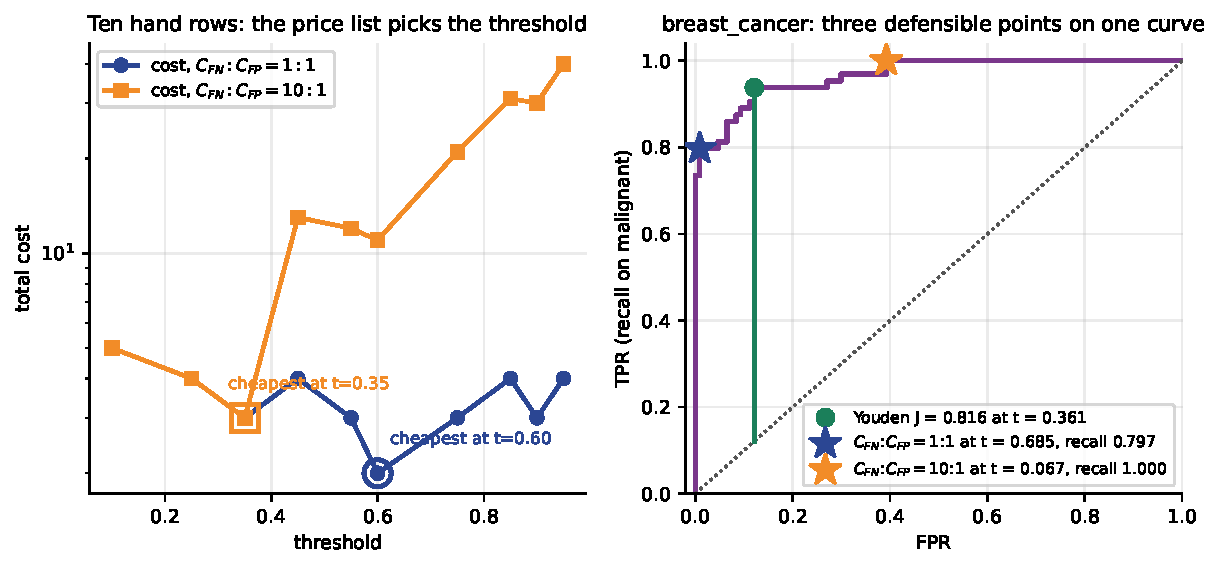
\includegraphics[width=0.80\textwidth]{l19-cost-threshold.pdf}
  \end{center}
  \begin{center}\small
    Left: total cost against threshold on the ten hand rows at $1\!:\!1$ and
    $10\!:\!1$; the minima are at $0.60$ and $0.35$. Right: three operating
    points on one \texttt{breast\_cancer} ROC curve. \textbf{The curve is the
    model; the points are decisions.}
  \end{center}
  \begin{alertblock}{The threshold is a parameter, and parameters leak}
    \footnotesize Maximising $J$, or minimising cost, \textbf{on the test set}
    is fitting to the test set --- the same error as choosing features on it,
    just smaller. Choose the threshold on a validation split or inside the
    folds; report once, at the threshold you already chose.
    \texttt{TunedThresholdClassifierCV} does exactly this inside a
    \texttt{Pipeline}.
  \end{alertblock}
\end{frame}

% =====================================================================
\section[Multiclass]{More than two classes}
\label{sec:multi}

\begin{frame}[shrink=9]{By hand: a hundred rows in three classes}
For class $i$: $\TP_i$ is the diagonal entry, $\FP_i$ is the rest of
\emph{column} $i$, $\FN_i$ is the rest of \emph{row} $i$.
  \begin{columns}[T]
    \begin{column}{0.42\textwidth}
      \begin{center}\small
      \begin{tabular}{@{}lrrrr@{}}
        \toprule
         & pred A & pred B & pred C & total\\
        \midrule
        actual A & $54$ & $4$ & $2$ & $60$\\
        actual B & $6$ & $21$ & $3$ & $30$\\
        actual C & $4$ & $2$ & $4$ & $10$\\
        \midrule
        col.\ total & $64$ & $27$ & $9$ & $100$\\
        \bottomrule
      \end{tabular}
      \end{center}
    \end{column}
    \begin{column}{0.55\textwidth}
      \begin{block}{The off-diagonal pattern is the informative part}
        \footnotesize A model that confuses $3$ with $8$ has a different
        problem from one that confuses $3$ with $5$. \textbf{No single average
        will tell you which.} Accuracy is the diagonal over the total:
        $(54 + 21 + 4)/100 = \mathbf{0.79}$.
      \end{block}
    \end{column}
  \end{columns}
  \vspace{0.2em}
  \begin{center}\footnotesize
  \begin{tabular}{@{}lrrrrrrr@{}}
    \toprule
    class & $\TP$ & $\FP$ & $\FN$ & support & precision & recall & $F_1$\\
    \midrule
    A & $54$ & $10$ & $6$ & $60$ & $54/64 = 0.843750$ & $0.900000$ &
      $0.870968$\\
    B & $21$ & $6$ & $9$ & $30$ & $21/27 = 0.777778$ & $0.700000$ &
      $0.736842$\\
    C & $4$ & $5$ & $6$ & $10$ & $4/9 = 0.444444$ & $0.400000$ &
      $0.421053$\\
    \bottomrule
  \end{tabular}
  \end{center}
\end{frame}

\begin{frame}[shrink=10]{By hand: micro, macro and weighted}
  \begin{columns}[T]
    \begin{column}{0.52\textwidth}
      \textbf{Micro} pools the counts before dividing:
      $\sum\TP = 79$, $\sum\FP = 21$, $\sum\FN = 21$, so micro precision
      $=$ recall $=F_1 = 79/100 = 0.79$.
      \begin{align*}
        \text{macro }p &= \tfrac{1}{3}(0.843750 + 0.777778 + 0.444444)
          = 0.688657\\
        \text{macro }r &= \tfrac{1}{3}(0.9 + 0.7 + 0.4) = 0.666667\\
        \text{macro }F_1 &= \tfrac{1}{3}(0.870968 + 0.736842 + 0.421053)\\
          &= 0.676287
      \end{align*}
      Weighted uses the supports $60, 30, 10$:
      \begin{align*}
        \text{wtd }F_1 &= \tfrac{60(0.870968) + 30(0.736842)
                                 + 10(0.421053)}{100}\\
                       &= 0.785739
      \end{align*}
    \end{column}
    \begin{column}{0.44\textwidth}
      \begin{block}{Two facts that fall out}
        \footnotesize \textbf{(1)} In single-label multiclass, micro precision,
        micro recall and micro $F_1$ all equal \emph{accuracy} --- always,
        because every row contributes exactly one $\TP$ or one $\FP$ and one
        $\FN$.\\[0.3em]
        \textbf{(2)} \textbf{Weighted recall equals accuracy}, always, because
        $\sum_i n_i(\TP_i/n_i) = \sum_i \TP_i$.
      \end{block}
      \begin{alertblock}{And the gap is the warning}
        \footnotesize Macro $F_1$ is $\mathbf{0.1095}$ \emph{below} weighted
        $F_1$, because class C is a tenth of the rows, a third of the macro
        vote, and the model is bad at it.
      \end{alertblock}
    \end{column}
  \end{columns}
\end{frame}

\begin{frame}[fragile,shrink=7]{The same hundred rows, in code}
\begin{lstlisting}
print(classification_report(y_true3, y_pred3, digits=6,
                            target_names=["A", "B", "C"]))
\end{lstlisting}
\begin{outblk}
              precision    recall  f1-score   support

           A   0.843750  0.900000  0.870968        60
           B   0.777778  0.700000  0.736842        30
           C   0.444444  0.400000  0.421053        10

    accuracy                       0.790000       100
   macro avg   0.688657  0.666667  0.676287       100
weighted avg   0.784028  0.790000  0.785739       100
\end{outblk}
\onslide<2->
\begin{exampleblock}{}
  \centering\small
  \textbf{Micro} asks ``how often is the model right?'' \textbf{Macro} asks
  ``how well does it do on a typical \emph{class}?'' \textbf{Weighted} asks
  ``how well does it do on a typical \emph{row}?'' Choose by deciding who you
  are answerable to: a per-class regulator wants macro, a throughput target
  wants micro.
\end{exampleblock}
\end{frame}

\begin{frame}[fragile,shrink=7]{On real data, where the rare classes hide}
\texttt{load\_digits} with two classes made rare on purpose --- only $20$
examples each of the digits $3$ and $8$.
\begin{outblk}
imbalanced digits: 1480 rows, class counts [178 182 177  20 181 182 181 179  20 180]
accuracy 0.9662
  micro     precision 0.9662  recall 0.9662  F1 0.9662
  macro     precision 0.9730  recall 0.9131  F1 0.9339
  weighted  precision 0.9669  recall 0.9662  F1 0.9652
per-class recall: [1.     0.9818 0.9811 0.8333 0.963  0.9273 0.9815 0.9815 0.5    0.9815]
classes 3 and 8 have 6 test rows each and recall 0.8333 and 0.5000.
micro hides them completely; macro is the only average that shows them.
\end{outblk}
\onslide<2->
\begin{center}\small
  Micro and weighted both read $0.97$. Macro reads $0.93$, and macro
  \emph{recall} reads $\mathbf{0.9131}$ --- because the model finds half
  of the eights. \textbf{If the eights are the cases you care about, only the
  macro row and the per-class array told you anything.}
\end{center}
\end{frame}

\begin{frame}[fragile,shrink=8]{Predict first \#5}
ROC needs a positive class, so multiclass ROC means $k$ one-vs-rest curves. A
three-class problem at roughly $80/15/5$; the model \textbf{never once
predicts class $2$}, so its recall and $F_1$ are $0.0000$.
\begin{center}
  \textbf{What is class $2$'s one-vs-rest AUC?}
\end{center}
\onslide<2->
\begin{outblk}
three classes, [709 140  51] in the test set
accuracy 0.8600

class  support   one-vs-rest AUC   recall      F1
  0        709          0.8920     0.9633  0.9236
  1        140          0.9090     0.6500  0.6766
  2         51          0.7793     0.0000  0.0000

macro    OvR AUC 0.8601   F1 0.5334
weighted OvR AUC 0.8883   F1 0.8328
micro                       F1 0.8600 (= accuracy 0.8600)
macro OvO AUC 0.8151

macro F1 0.5334 against weighted F1 0.8328: a gap of 0.2994.
Report the one that matches who you will disappoint.
\end{outblk}
\onslide<3->
\begin{alertblock}{Recall $0.0000$, $F_1$ $0.0000$, \textbf{AUC $0.7793$}}
  \footnotesize There is real information in the scores for class $2$;
  \texttt{argmax} simply never lets it win, because class $0$ is sixteen times
  as common and the prior buries it. \textbf{AUC sees the ranking; $F_1$ sees
  only the decision.} Report weighted $F_1 = 0.8328$ and stop, and you ship a
  model that cannot detect one of its three classes.
\end{alertblock}
\end{frame}

\begin{frame}[shrink=8]{Drawn: three curves, and the averaging choice}
  \begin{center}
    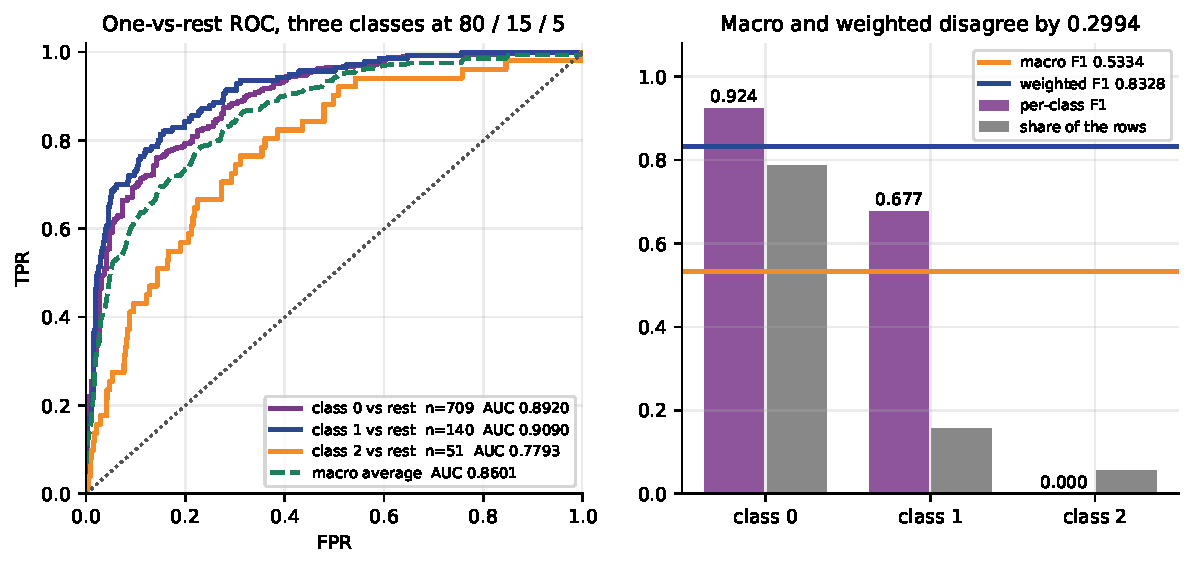
\includegraphics[width=0.86\textwidth]{l19-multiclass-ovr.pdf}
  \end{center}
  \begin{center}\small
    Left: three one-vs-rest ROC curves and their macro average. Right:
    per-class $F_1$ against class share, with macro and weighted as horizontal
    lines --- \textbf{they differ by $0.2994$.} There is also
    \texttt{multi\_class="ovo"}, averaging all $\binom{k}{2}$ pairwise AUCs
    ($0.8151$ here), which is the more natural choice when the class sizes are
    wildly different. \textbf{Report the average that matches who you will
    disappoint.}
  \end{center}
\end{frame}

% =====================================================================
\section[Selection]{Model selection, done properly}
\label{sec:selection}

\begin{frame}[fragile,shrink=8]{Seven classifiers, twenty folds, one metric}
\begin{lstlisting}
cv = RepeatedStratifiedKFold(n_splits=5, n_repeats=4, random_state=0)
res = {n: cross_val_score(m, Xb, yb, cv=cv, scoring="roc_auc")
       for n, m in models.items()}
\end{lstlisting}
\begin{outblk}
breast_cancer, all 30 features, 5-fold x 4 repeats = 20 folds
model             mean AUC     sd   2 s.e.    worst    best
SVM (RBF)         0.9950  0.0058  0.0026   0.9771  1.0000
Logistic reg.     0.9948  0.0056  0.0025   0.9803  1.0000
MLP (100)         0.9944  0.0060  0.0027   0.9800  1.0000
Random forest     0.9905  0.0090  0.0040   0.9705  1.0000
Gaussian NB       0.9882  0.0069  0.0031   0.9705  0.9993
KNN (k=5)         0.9849  0.0107  0.0048   0.9633  1.0000
Decision tree     0.9227  0.0205  0.0092   0.8809  0.9554
\end{outblk}
\onslide<2->
\begin{center}\small
  Three notes on the machinery. \texttt{RepeatedStratifiedKFold} gives twenty
  estimates rather than five, which is what makes the standard error worth
  quoting. \textbf{Every scaler sits inside a \texttt{Pipeline}}, so it is
  refitted in each fold. And \texttt{scoring="roc\_auc"} was chosen
  \emph{before} the run, not after looking at the results.
\end{center}
\end{frame}

\begin{frame}[fragile,shrink=8]{Predict first \#6}
The table above is easy to read as a ranking: SVM (RBF) $0.9950$ beats
logistic regression $0.9948$.
\begin{center}
  \textbf{Is that a result? How many of the twenty folds did the SVM actually
  win?}
\end{center}
\onslide<2->
\begin{outblk}
best   SVM (RBF)        0.9950
second Logistic reg.    0.9948
gap 0.0003;  fold-to-fold sd of the gap 0.0022
paired t = 0.598, p = 0.5569 over 20 folds
SVM (RBF) beat Logistic reg. on 7 of the 20 folds
\end{outblk}
\onslide<3->
\begin{alertblock}{$0.9950$ against $0.9948$ is not a result}
  \footnotesize The lead is $0.0003$. The fold-to-fold standard deviation of
  that lead is $0.0022$, \textbf{seven times larger}, and the nominal winner
  \emph{lost thirteen of the twenty folds}. A paired $t$-test gives
  $p = 0.5569$. \textbf{When the gap is smaller than the noise, choose on
  something else:} training time, interpretability, behaviour on the tail,
  whether you can explain it to a clinician.
\end{alertblock}
\end{frame}

\begin{frame}[fragile,shrink=8]{The ranking flips from fold to fold}
\begin{outblk}
fold-by-fold, the top four models, first eight folds
fold  SVM (RBF)      Logistic reg.  MLP (100)      Random forest  winner
  0   0.9869         0.9846         0.9840         0.9813         SVM (RBF)
  1   0.9987         0.9990         0.9954         0.9990         Logistic reg.
  2   0.9967         0.9980         0.9974         0.9866         Logistic reg.
  3   1.0000         1.0000         1.0000         0.9964         SVM (RBF)
  4   0.9963         0.9956         0.9946         0.9980         Random forest
  5   0.9925         0.9905         0.9889         0.9880         SVM (RBF)
  6   0.9977         0.9987         0.9984         0.9838         Logistic reg.
  7   0.9983         0.9950         0.9997         0.9960         MLP (100)
\end{outblk}
\onslide<2->
\begin{center}\small
  \textbf{Four different winners in eight folds.} Had you run a single
  $80/20$ split you would have crowned one of them, and which one would have
  been decided by \texttt{random\_state}.
\end{center}
\end{frame}

\begin{frame}[fragile,shrink=10]{Drawn: error bars, and every fold}
  \begin{center}
    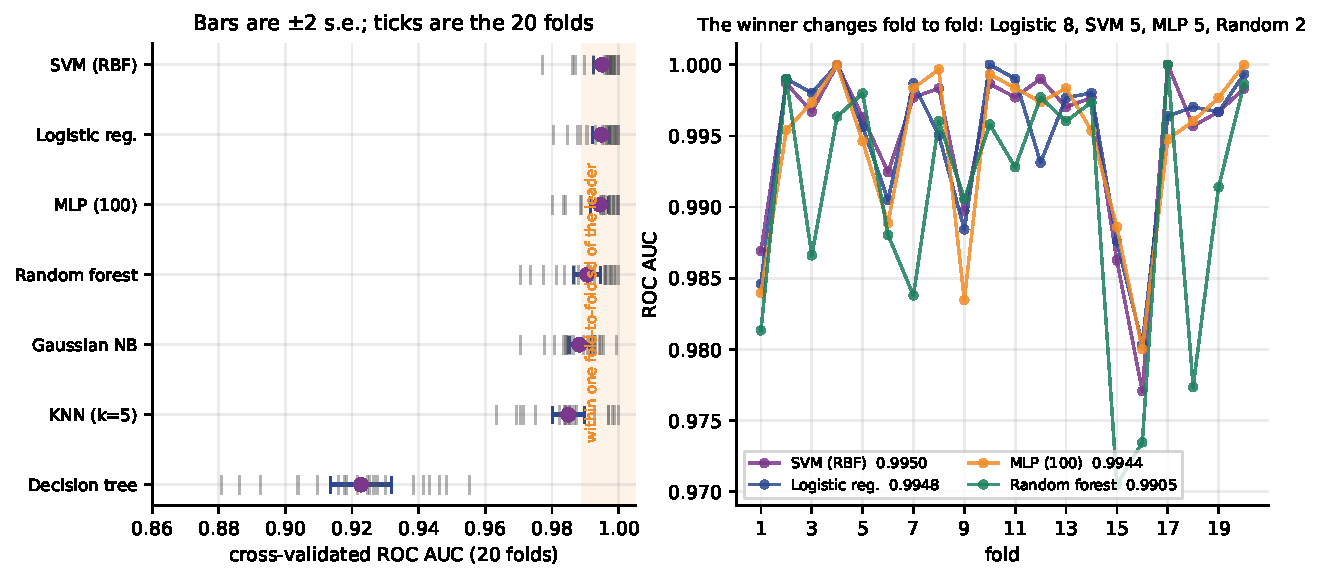
\includegraphics[width=0.72\textwidth]{l19-model-selection.pdf}
  \end{center}
\begin{outblk}
fold-to-fold sd of the leader: 0.0058
models within one sd of the leader: Logistic reg., MLP (100), Random forest, SVM (RBF)
A gap smaller than the fold-to-fold spread is not a difference.
\end{outblk}
  \begin{center}\small
    Left: mean cross-validated AUC with $\pm 2$ standard-error bars; the ticks
    are the twenty individual folds and the band is one fold-to-fold standard
    deviation of the leader. Right: the top four models fold by fold ---
    \textbf{the lines cross constantly}, and \textbf{six of the seven models
    won at least one fold}.
  \end{center}
\end{frame}

\begin{frame}[fragile,shrink=8]{And the metric decides the ranking}
The same seven models, the same folds, scored by accuracy as well as AUC.
\begin{outblk}
the same seven models scored by accuracy and by AUC, same folds
model             accuracy     AUC    acc rank   AUC rank
SVM (RBF)         0.9771    0.9957       3          1
Logistic reg.     0.9789    0.9955       1          2
MLP (100)         0.9789    0.9943       2          3
Random forest     0.9578    0.9923       5          4
Gaussian NB       0.9385    0.9885       6          5
KNN (k=5)         0.9649    0.9806       4          6
Decision tree     0.9262    0.9210       7          7
models whose rank differs between the two metrics: 6 of 7
Pick the metric before you pick the model, and say why.
\end{outblk}
\onslide<2->
\begin{alertblock}{Six of seven models change rank}
  \footnotesize $k$-NN is fourth by accuracy and sixth by AUC; the random
  forest is fifth by accuracy and fourth by AUC. \textbf{There is no
  metric-free notion of ``the best model''} --- which closes the loop with the
  first section, where accuracy and AUC ranked two models in opposite orders.
\end{alertblock}
\end{frame}

\begin{frame}[shrink=6]{The checklist for your classifier comparison}
  \begin{columns}[T]
    \begin{column}{0.48\textwidth}
      \begin{enumerate}\small
        \item State the \textbf{positive class} and the \textbf{prevalence}.
        \item State the metric \emph{before} you run anything, and say why
          that metric.
        \item Put every preprocessing step inside a \texttt{Pipeline}.
        \item Use \textbf{repeated stratified cross-validation}, not one
          split.
        \item Report mean, standard deviation and the number of folds ---
          never a mean alone.
      \end{enumerate}
    \end{column}
    \begin{column}{0.48\textwidth}
      \begin{enumerate}\small
        \setcounter{enumi}{5}
        \item Include a baseline: \texttt{DummyClassifier}, and one simple
          model.
        \item Plot the ROC curves together, and the PR curves too if positives
          are rare.
        \item Choose the threshold from a stated cost or capacity constraint,
          \textbf{on validation data}.
        \item Say plainly when two models are indistinguishable, and give the
          \emph{non-statistical} reason you picked one.
      \end{enumerate}
    \end{column}
  \end{columns}
  \vspace{0.2em}
  \begin{alertblock}{}
    \centering\small
    Nine lines. \textbf{Every one of them is a mark on the assignment, and
    eight of them are one sentence in your report.}
  \end{alertblock}
\end{frame}

% =====================================================================
\section{Summary}
\label{sec:summary}

\begin{frame}[shrink=17]{Summary --- eleven lines}
  \begin{enumerate}\small
    \item Accuracy is a weighted summary and the weights are the class
      frequencies. At $1\%$ prevalence a constant predictor scored
      $\mathbf{0.9900}$ and a useful logistic regression scored
      $\mathbf{0.9897}$ --- \textbf{accuracy ranked them backwards} while AUC
      ranked them $0.5000$ against $0.9200$.
    \item Four counts, six metrics. On twenty patients with $\TP = 6$,
      $\FP = 2$, $\FN = 4$, $\TN = 8$: accuracy $0.7000$, precision $0.7500$,
      recall $0.6000$, specificity $0.8000$, $\FPR = 0.2000$,
      $F_1 = 0.6667$ --- and \texttt{confusion\_matrix} is the
      \emph{transpose} of the textbook layout.
    \item A classifier outputs a score and \texttt{predict} silently
      thresholds it. One fixed set of scores gave accuracies from $0.7135$ to
      $0.9181$ across seven thresholds, \textbf{with AUC fixed at $0.9661$
      throughout}.
    \item An ROC curve is a sorted list and some bookkeeping: up $1/P$ for a
      positive, right $1/N$ for a negative. The eleven-point hand sweep
      matched \texttt{roc\_curve(drop\_intermediate=False)} exactly; the
      default keeps $8$ of the $11$ points and the same area.
    \item AUC two ways, same answer. Trapezoids
      $0.08 + 0.16 + 0.16 + 0.20 + 0.20 = \mathbf{0.80}$; concordant pairs
      $\mathbf{20/25 = 0.80}$. It is the probability a random positive
      outranks a random negative, and the Mann--Whitney $U$ rescaled. All
      $6848$ pairs on \texttt{breast\_cancer} matched \texttt{roc\_auc\_score}
      to $0.00\mathrm{e}{+}00$.
    \item AUC $0.5$ is chance --- $200$ coin-flip runs gave mean $0.4994$,
      sd $0.0136$, max $0.5342$. Below $0.5$ is an \emph{inverted} classifier:
      $0.9661$ becomes $0.0339$, and $\mathrm{AUC}(-s) = 1 - \mathrm{AUC}(s)$
      exactly.
    \item AUC is invariant to the threshold by construction and to the class
      balance by measurement: over a fiftyfold change in prevalence it moved
      inside a band of $0.0085$ while average precision moved
      $0.1702 \to 0.9202$.
    \item \textbf{Under heavy imbalance ROC flatters.} ROC AUC $0.9200$,
      average precision $0.1702$; at $90\%$ recall that is $1156$ false alarms
      for $54$ true ones --- one alert in twenty-two. \textbf{The PR baseline
      is the prevalence, not $0.5$.}
    \item The threshold is a business decision. Ten hand rows: $1\!:\!1$ picks
      $0.60$ (recall $0.80$), $10\!:\!1$ picks $0.35$ (recall $1.00$). On
      \texttt{breast\_cancer}, $1\!:\!1 \to 10\!:\!1$ moved the threshold
      $0.6855 \to 0.0670$, misses $13 \to 0$, false alarms $1 \to 42$.
      Youden's $J$ is the equal-cost answer in disguise.
    \item Multiclass: micro always equals accuracy, weighted recall always
      equals accuracy, macro gives the rarest class a full vote. Hand example:
      macro $F_1$ $0.676287$ against weighted $0.785739$. And a class with
      $F_1 = 0.0000$ had a one-vs-rest \textbf{AUC of $0.7793$}.
    \item Model selection: the best two of seven differed by $\mathbf{0.0003}$
      with a fold-to-fold spread of $\mathbf{0.0058}$, $p = 0.5569$, the
      leader losing $13$ of $20$ folds, and \textbf{six of seven models
      changing rank} when the metric changed. \textbf{A difference smaller
      than the fold-to-fold spread is not a difference.}
  \end{enumerate}
\end{frame}

\begin{frame}[shrink=4]{Before the assessment session}
  \begin{columns}[T]
    \begin{column}{0.48\textwidth}
      \begin{block}{Read}
        \texttt{notes.pdf} --- the full development, the sampling check on
        the AUC identity, the leakage argument for thresholds, and
        \textbf{10 practice questions with worked solutions}.
      \end{block}
      \begin{block}{Do}
        Questions 1, 2, 3, 5 and 7, \textbf{with a pen}. Question 3 is an
        eight-row ROC sweep with the AUC computed both ways; question 5 costs
        the same eight rows at $8\!:\!1$; question 7 is the multiclass
        averaging.
      \end{block}
    \end{column}
    \begin{column}{0.48\textwidth}
      \begin{exampleblock}{This closes the classification unit}
        The next test covers neural networks, support vector machines and
        \textbf{this lecture}, and the ROC sweep is the numeric question most
        likely to appear. The assignment that follows is a
        \textbf{classifier comparison with ROC and AUC} --- the nine-line
        checklist two frames back is its marking scheme in disguise.
      \end{exampleblock}
      \begin{alertblock}{One habit to start now}
        Never quote an accuracy without saying \textbf{what the baseline
        scores} and \textbf{what threshold you used}. If you cannot answer
        both, you have not evaluated anything.
      \end{alertblock}
    \end{column}
  \end{columns}
  \begin{center}
    \small Materials: \texttt{\AMLRepoURL}
  \end{center}
  \slidesources{\AMLUnitVISources}
\end{frame}

\end{document}
